\section{Smerte}
\textit{Dette afsnit omhandler smerte hvor de anatomiske og fysiologiske egenskaber vil beskrives. Herunder vil de forskellige kategorier af smerte forklares, og hvilken sammenhæng de har til kroniske smerter.}


\textbf{Dette afsnit skal skrives sammen med det foregående}
Operationer udføres ofte for at gøre patienten fri for smerte. Der opstår derfor et klart problem når patienten behandles, men smerterne fortsætter eller forværres. Hos TKA patienter opleves det i 19\% af alle tilfælde efter operation \citep{Petersen2015}. Her oplever 19\% af patienter efter den primære operation, og 47\% af patienter efter revision af operationen svære til uudholdelige smerter. Dette sker på trods af at der i hele Danmark udføres knæoperationer som alle signifikant overholder indikationerne for behandlingskvaliteten samt at kvaliteten er stigende \citep{aarsrapport2016}. Dette antyder, at patienternes smerter ikke skyldes fejl ved operationen.


\subsection{Smertes anatomi eller fysiologi}
Smerte er defineret som: “\textit{An unpleasant sensory and emotional experience associated with actual or potential tissue damage, or described in terms of such damage.}” af The International Association for the Study of Pain (IASP) \citep{Giangregorio1997}, \citep{Carmon}.\\
Selvom smerte normalt er en følelse, der forsøges undgået, er det en nødvendig del af menneskets overlevelse. Det fortæller kroppen om farer eller skader som skal reageres på, så yderligere skade kan undgås.
% \textbf{Tilføj hvilke aktiveringsveje smerten har, hvilke stoffer der benyttes etc.}
Smerte er en oplevelse hjernen har når den modtager stimuli fra neuroner i kroppen. Oplevelsen kaldes perception af smerte og er forskellig fra sensationen af smerte. Sensationen sker idet neuroner stimuleres og genererer et aktionspotentiale. Perceptionen sker først når impulsen når til hjernen, og hjernen opfatter smerten. 

%smerte i martini: ca 500 og frem
%Nerveimpuls: aktionspotentiale generering, impuls langs nerve, fra nerve til nerve
%nervesignalets vej fra fx finger til rygmarv: nerveimpuls fra nerve til rygmarv (ganglia, plexus)
%refleks funktionen i rygmarven (refleks pga sensation sker før perception og beslutningstagen i hjernen)
%	[evt nyt afsnit]
%smerte perception i hjernen -> typer af smerte (hvor kommer smerten fra? er det skade på væv (er det således nociceptisk (somatisk/visceral(referredpain)) eller neuropatisk?) eller psykogen?)

Smerter registreres af neuroner i kroppen. De fleste smertereceptorer er frie neuronender som forgrener sig ud i hele kroppen, og ligger frit i væv. De dækker således et stort område og kan reagere på forskellige typer stimuli som vævet bliver udsat for. Typen af stimuli bliver bestemt afhængig af hvilke porte som aktiveres på neuronerne. De besidder forskellige typer af natrium-/kaliumporte, som aktiveres ved temperaturændring, trykforandring og kemisk foranding, som ses på figur \ref{neuronport}.

\begin{figure}[H] 
	\begin{center}
	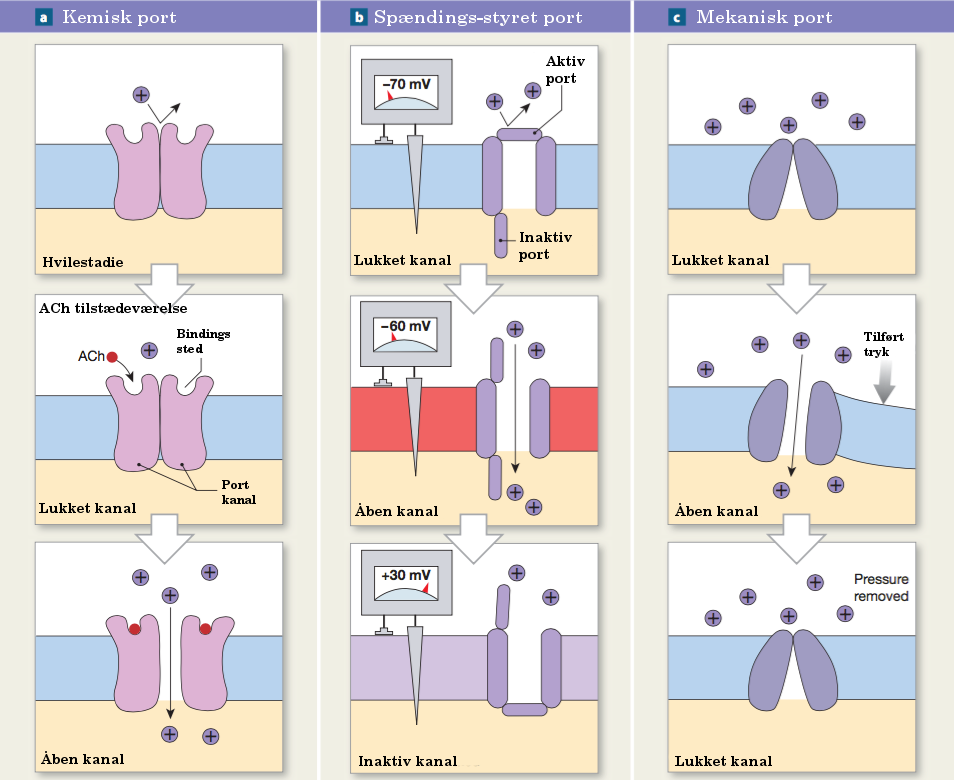
\includegraphics[width=0.5\textwidth]{figures/neuronport}
	\end{center}
		\caption{Neuronporte \citep{Martini}}
		\label{neuronport}
		\centering
\end{figure}

Termoreceptorer er ikke illustreret på figur \ref{neuronport}, men fungerer ved at proteinerne som portene består af, åbner sig ved bestemte temperaturer og derved lader natrium og kalium passere igennem \citep{kimball}. 
Når en eller flere af disse typer porte åbner strømmer natrium ind i neuronet, mens kalium strømmer ud, og neuronets membranpotentiale stiger. Et gradientpotentiale opbygges og hvis dette er tilstrækkelig højt opnås neuronets tærskelværdi, og et aktionspotentiale sendes afsted. Dette potentiale når til en synapsespalte mellem to neuroner, hvor potentialet overføres ved frigivelse af kemiske transmitterstoffer, som acetylcholin (ACh). Modtagerneuronet har ACh recptorer som igangsætter opbygningen af et gradientpotentiale, så impulsen kan fortsætte. \\
Impulsen fortsætter ad neuronerne til en dorsal ganglion, hvor flere neuroner samles inden de ledes ind i henholdsvis rygmarvens spinothalamiske tragt eller den posteriore søjle, afhængig af om de bringer information om upræcis berøring, tryk, temperatur og smerte, eller præcis berøring, vibration og proprioception. \citep{Martini}

%sendes til centralnervesystemet (CNS), hvor det først når rygmarven og lidt senere hjernen. Her skelnes der mellem smerte sensation og perception. Smertesensation er information om smerte, som nerverne i hånden der registrere den skadelige temperatur. Smerte perceptionen sker først når nervesignalet når op til hjernen og denne modtager signalet og opfatter det som smerte. Sensationen af smerte kan i rygsøjlen aktivere en refleks der får musklerne i armen til at trække hånden væk fra varmen, inden hjernen når at registrere og opfatte den egentlige smerte. \citep{Martini} Denne form for smerte er kategoriseret som akut-nødvendig smerte, da det hjælper kroppen med at undgå skader.

\subsection{Smertetyper}
%Modsat akut-nødvendig smerte findes unødvendig smerte. Denne smerte kaldes også kronisk smerte, da den oftest er længerevarende, ved at have været konstant i mindst tre måneder \citep{Giangregorio1997}. 

% kilde der siger at nociceptisk smerter både er akut og kronisk: http://www.slideshare.net/ssakpi/molecular-mechanisms-of-pain-part-1
% kilde der siger at akut og kronisk smerte er to helt forskellige ting, hvor nociceptisk og neuropatisk begger er under kronisk: http://www.denalihealthcaremi.com/tag/classification-of-pain/
% kilde som siger at smerte kan opdeles efter hvordan det bestemmes: udfra længde af smerten eller udfra smertens natur (oprindelse)
% hvis man skære en nerve over, burde smerten kunne kategoriseres som akut, men idet det er en skade på en nerve er det neuropatisk og derfor kronisk smerte?

Der findes flere måder at opdele og kategorisere smerte på, men generelt kan det opdeles i to overordnede kategorier; akut og kronisk. \\
\textbf{Her skal indsættes en figur (stamtræ) med de forskellige typer af smerter} 
Hver kategori har flere undergrupperinger, hvor det er omdiskuteret hvordan disse grupper skal placeres. \citep{Giangragorio1997} På figur \ref{smertediagram} er en oversigt over, hvordan smerten kategoriseres i dette projekt.

\begin{figure}[H]
	\caption{smertediagram}
	\label{smertediagram}
	\centering
	\includegraphics[scale=.8]{figures/smertediagram}
	\flushleft
	\textit{SOURCE?}
\end{figure}

\subsubsection{Akut smerte}
Akut smerte er en nødvendig smerte, som fortæller hjernen om øjeblikkelig vævsskade, så kroppen hurtigt kan afværge dette. Akut smerte forårsages af traumer i eller på kroppen, og der skelnes herunder mellem to typer af smerte: nociceptisk og neuropatisk. Nociceptisk smerte udløses af skade på væv, herunder indre organer, overflader af kroppen og knogler. Nociceptisk smerte skyldes aktivering af nociceptorer, som oftest sidder som frie neuronender i væv. Som tidligere beskrevet er de følsomme overfor temperaturændringer, mekanisk stimuli eller kemiske ændringer, og kan derved aktiveres på mange måder. Da nociceptorer både er inde i og uden på kroppen, opdeles nociceptisk smerte i somatisk og visceral smertesensation. Somatisk smertesensation er information fra det \textit{yderste} af kroppen. Det er således sensation fra hud og muskulaturer i overfladen af torso, hoved, hals og lemmer. \citep{Martini} Smerten er øjeblikkelig og let placerbar. \\
Visceral smertesensation er information fra de indre organer i hals og abdomen. Sensation herfra opfattes sjældent, da de fleste indtryk er unødvendige at tage stilling til. Hvis der i midlertid opstår smerter i disse områder er denne besværlig at placere. Smerten er typisk ikke øjeblikkelig, men mere trykkende og langvarig; mavesmerter er et eksempel på visceral smerte. \\
Fordi viscerale og somatiske neuroner deles om rygmarvens spinothalamiske tragt, kan visceral information fra indre organer blive opfattet som somatisk information ved forskudt smerte. Smerte på grund af skade i indre organer vil derfor typisk opfattes som somatiske smerter. Ved forskudt smerte kan smerte i venstre arm og skulder således være forårsaget af smerte i hjertet.

\begin{figure}[H]
\begin{center}
\includegraphics[width=0.4\textwidth]{figures/forskudtsmerte}
	\caption{Forskudt smerte \citep{Martini}}
	\label{forskudtsmerte}
\end{center}
\end{figure}


Nociceptisk smerte er oftest ikke årsag til kroniske smerter, med mindre smerterne bliver ved.\\ 
Neuropatisk smerte opstår af skader på nervesystemet selv, herunder neuroner, rygmarv, neural plexus eller hjernen. 
Ved neuropatisk smerte registrer neuronerne et stimuli, som kan skyldes infektioner og sygdomme som iskæmi, sclerose, diabetes og kræft. Disse stimuli kan ligeledes være forårsaget af traumer fra smerter som startede med at være nociceptiske. Dette stimuli kan, afhængigt af hvor de påvirkede neuroner er lokaliseret, resultere i forskellige former for neuropatisk smerte. Smerten kan opleves som konstant og langvarig, hvor et typisk eksempel er fantomsmerter, men kan også være lejlighedsvis som ved hyperalgesi, hvor almindelig berøring opfattes som smertefuldt. \citep{Giangregorio1997}, \citep{Carmon}.

\subsubsection{Kronisk smerte}
Modsat akut smerte er kronisk smerte en længerevarende oplevelse af smerte. Det er af IASP defineret som at være smerteperception som varer længere end det generelt ville forventes \citep{Carmon}. Ofte sættes denne grænse ved tre måneder, men i nogle kliniske undersøgelser, eller hos nogle kræftpatienter kan smerten allerede efter en måned kategoriseres som værende kronisk. Som det kan ses af \figref{smertediagram} hænger akut og kronisk smerte sammen ved organisk smerte. Dette skyldes, at kronisk smerte ofte opstår på baggrund af en akut smerte, som, mod forventningen, ikke stopper. Kronisk smerte kan således opleves af en person som har oplevet enten nociceptisk eller neuropatisk smerte, hvis vedkommende efter heling stadig har smerter. Kronisk smerte kan ligeledes være af psykogen oprindelse.\\
Psykogene smerter er, til forskel fra nociceptisk og neuropatisk smerte, ikke en egentlig skade på kroppens væv. Det er en imaginær perception af smerte, og derved den mest besværlige at præcisere, idet der ikke er og muligvis aldrig har været en fysisk årsag til smerten. Hos en person med psykogene smerter er hjernen fuldt overbevidst om, at den oplever fysiske, nociceptiske eller neuropatiske, smerter og lider deraf. Smerten er udelukkende psykisk hos personen, men er af den grund ikke mindre virkelig, grundet smertes subjektive natur. \citep{Giangregorio1997}

%\subsection{Problemet ved kronisk smerte og operationer}
%Der findes således flere forskellige former for smerte, hvor kun nogle få er beskrevet her \cite{Carmon}. Alle kan de lede til kronisk smerte. Man ved derfor godt hvad der kan give kronisk smerte, hvordan smerten opfattes og hvor i kroppen den kommer fra. Men man ved endnu ikke hvorfor kronisk smerte opstår. Hvorfor føler kroppen fantom smerter fra et legeme som ikke er der? Hvorfor registrere hjernen smerte fra indre organer, når der intet er i vejen med dem? 



